\documentclass[10pt]{beamer}

% \usepackage{beamerthemesplit} // Activate for custom appearance
\usepackage{amsmath}
\usepackage{bookmark}
\usepackage{multirow}
\usepackage{xcolor,colortbl}
\definecolor{Gray}{gray}{0.9}
\usepackage[load=accepted]{siunitx}

\title{Piston error induced by mount trajectories}
\author{GMTO IM Group}
\date{\today}

% - - - - - - - - - - - - - - - - - - - - - - - - - - - - - - - - - - - - - - - 
\begin{document}

\frame{\titlepage}

%\section[Outline]{}
%\frame{\tableofcontents}


% - - - - - - - - - - - - - - - - - - - - - - - - - - - - - - - - - - - - - - - 
\section{Preamble}
% - - - - - - - - - - - - - - - - - - - - - - - - - - - - - - - - - - - - - - - 
\frame
{
  \frametitle{Initial considerations}
  \begin{enumerate}
  \item The telescope integrated model considers the PDR2021 mount subsystem design.
  \item We computed the piston error using a performance matrix transformation (PMT2) and through the GMTO's linear optical model (LOM) fed by the M1 and M2 rigid-body motions.
  \item Besides the baseline rejection transfer function (RTF) referred to as AGWS, we evaluate three variants obtained with the on-instrument wavefront sensor (OIWFS) outer control loop corresponding to different update rates: OIWFS-10 (\SI{10}{Hz}), OIWFS-50 (\SI{50}{Hz}), and OIWFS-125 (\SI{125}{Hz}).
  \item We evaluate three trajectories among those in GMT-DTA-193917: TJ101, TJ102, and TJ103. The first two are critical cases, with the telescope elevation close to the zenith, leading to higher accelerations. The third is a milder case, departing from $\approx$\SI{30}{deg}. The simulations with the first two trajectories consider the model linearized at \SI{0}{deg} elevation. For TJ103, the plant model reproduces the behavior around \SI{30}{deg}.
  \end{enumerate}
  
}

% - - - - - - - - - - - - - - - - - - - - - - - - - - - - - - - - - - - - - - - 
\section{LTAO Piston RTF}
% - - - - - - - - - - - - - - - - - - - - - - - - - - - - - - - - - - - - - - - 
\begin{frame}{LTAO Piston RTF variants}
  The LTAO differential piston rejection transfer function (RTF) reads as
  $$
    H_\text{dp-rtf}(s) = \frac{1 - \left(1 -e^{-T_e s}\right)\dfrac{4\pi^2 f_z^2 g_\text{eff} e^{-\tau_e s} }{T_e s \left(4\pi^2 f_z^2 + 4\pi \delta_z f_z s + s^2\right)}}
    {1 +\left(1 -e^{-T_p s}\right)\dfrac{4\pi^2 f_z^2 g_\text{pi} e^{-\tau_p s} }{\left(T_p s\right)^2 \left(4\pi^2 f_z^2 + 4\pi \delta_z f_z s + s^2\right)}} ,
  $$
where $f_z=\SI{800}{Hz}$, $\delta_z=0.75$, $g_\text{pi}=0.5$, $T_e=\SI{2}{ms}$, and $g_\text{eff}=0.8$. The other parameters assume different values according to the variants presented below.
  \begin{center}
  \begin{tabular}{l|ccccc}
  RTF & $T_p$ & $\tau_p$ & $\tau_e$ \\ \hline
  AGWS & \SI{30}{s} & \SI{6}{ms} & \SI{0.1}{ms}\\
  OIWFS-10 & \SI{0.1}{s} & \SI{50}{ms} & \SI{0.2}{ms}\\
  OIWFS-50 & \SI{0.02}{s} & \SI{10}{ms} & \SI{0.2}{ms}\\
  OIWFS-125 & \SI{0.008}{s} & \SI{10}{ms} & \SI{0.2}{ms}
  \end{tabular}  
  \end{center}
  
\end{frame}



\begin{frame}{Piston RTF variants comparison}
  The next figure shows the magnitude response of the RTFs.
  \begin{center}
  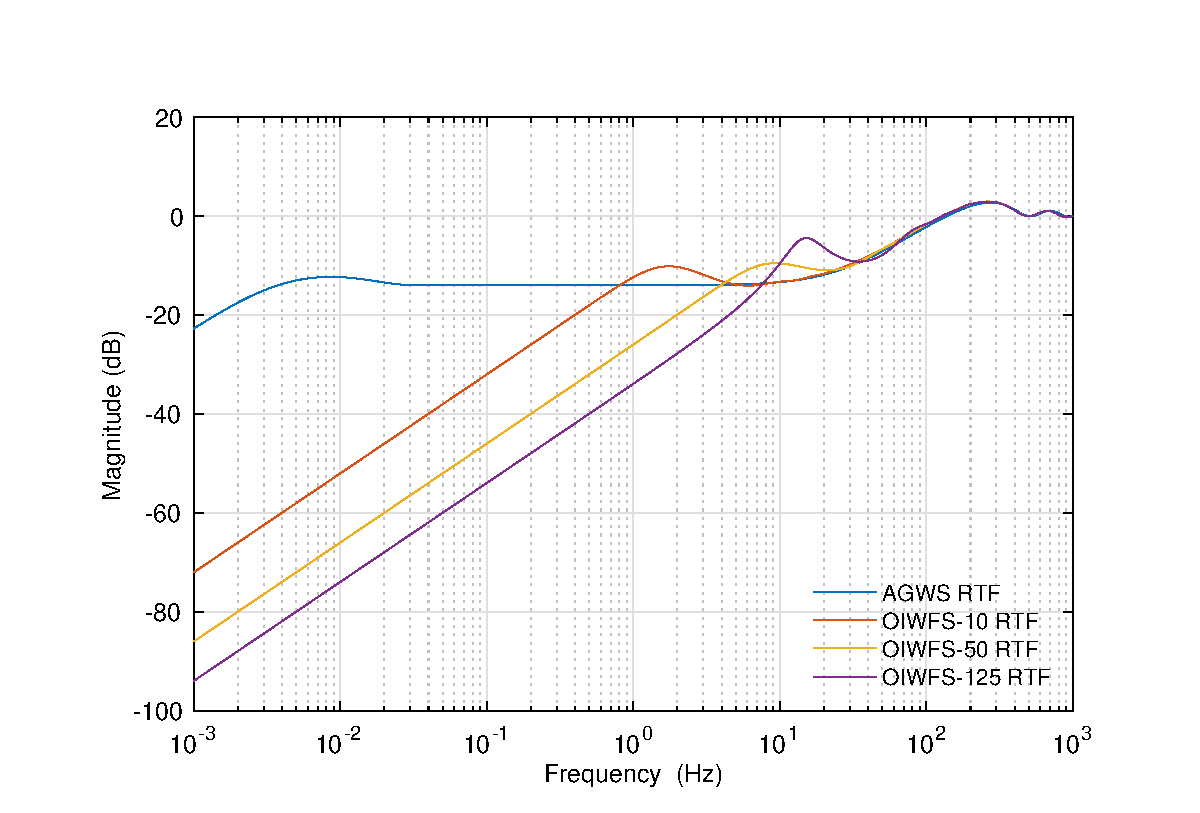
\includegraphics[width=\textwidth]{rtf_variants.eps}      
  \end{center}
\vfill
\end{frame}


% - - - - - - - - - - - - - - - - - - - - - - - - - - - - - - - - - - - - - - - 
\section{Results \& Comments}
% - - - - - - - - - - - - - - - - - - - - - - - - - - - - - - - - - - - - - - - 
\begin{frame}{Simulation Results: piston error}
  %\small
  \begin{center}
  \begin{tabular}{l l|cccc}
    & & AGWS & OIWFS-10 & OIWFS-50 & OIWFS-125 \\
   \hline \rowcolor{Gray}
   \multirow{2}{*}{TJ101} & PMT2 & \SI{23.3}{nm} & \SI{6.23}{nm} & \SI{5.42}{nm} & \SI{2.39}{nm} \\
                          & LOM & \SI{26.9}{nm} & \SI{15.9}{nm} & \SI{14.7}{nm} & \SI{6.56}{nm}\\
   \hline \rowcolor{Gray}
   \multirow{2}{*}{TJ102} & PMT2 & \SI{23.3}{nm} & \SI{6.23}{nm} & \SI{5.41}{nm} & \SI{2.39}{nm}\\
                          & LOM & \SI{27.0}{nm} & \SI{15.8}{nm} & \SI{14.7}{nm} & \SI{6.54}{nm}\\
   \hline \rowcolor{Gray} 
   \multirow{2}{*}{TJ103} & PMT2 & \SI{0.25}{nm} & \SI{0.178}{nm} & \SI{0.233}{nm} & \SI{0.25}{nm}\\
                          & LOM & \SI{0.57}{nm} & \SI{0.42}{nm} & \SI{0.395}{nm} & \SI{0.355}{nm}
  \end{tabular}  
  \end{center}
\end{frame}



% - - - - - - - - - - - - - - - - - - - - - - - - - - - - - - - - - - - - - - - 
\section{Concluding Remarks}
% - - - - - - - - - - - - - - - - - - - - - - - - - - - - - - - - - - - - - - - 
\begin{frame}{Concluding Remarks}
\begin{itemize}
  \item The simulations indicate that the RTFs representing the updated wavefront control architecture reduces significantly the piston error induced by the mount acceleration.
  \item The trajectory-induced piston error obtained from the LOM is systematically higher than those provided by the PMT2. The LOM optical measures the errors with respect to a fixed reference frame: the support structure (OSS) coordinate system. In contrast, PMT2 outputs incorporate the AGWS motion, which in turn, at least partially, follows the mount motion. In addition, the dynamics of the M1 segments, present only in the GMTO FE model, may also contribute to wavefront error differences. Therefore, the higher LOM-based numbers are not surprising.
\end{itemize}  
\end{frame}

\end{document}
